
\documentclass[11pt]{article}
\usepackage[a4paper,margin=1in]{geometry}
\usepackage{amsmath,amssymb}
\usepackage{graphicx}
\usepackage[dvipsnames]{xcolor}
\usepackage{hyperref}
\usepackage{enumitem}
\usepackage{tabularx}
\usepackage{longtable}
\usepackage{booktabs}
\usepackage[most]{tcolorbox}
\usepackage{titlesec}
\usepackage{xurl}
\usepackage{fancyhdr}
\usepackage{setspace}
\usepackage{tikz}
\usetikzlibrary{positioning,arrows.meta}
\usepackage[T1]{fontenc}
\usepackage{lmodern}
\setlength{\parindent}{0pt}
\setlength{\parskip}{8pt}
\setlength{\headheight}{14pt}
\setstretch{1.12}
\setlist[itemize]{leftmargin=1.5em, nosep}
\setlist[enumerate]{leftmargin=1.5em, nosep}
\providecommand{\tightlist}{\setlength{\itemsep}{0pt}\setlength{\parskip}{0pt}}
\hypersetup{colorlinks=true,linkcolor=MidnightBlue,urlcolor=MidnightBlue}
\pagestyle{fancy}
\fancyhf{}
\rhead{\thepage}
\renewcommand{\headrulewidth}{0pt}
\renewcommand{\footrulewidth}{0pt}
\titleformat{\section}{\Large\bfseries\color{MidnightBlue}}{\thesection}{0.6em}{}
\titleformat{\subsection}{\bfseries}{}{0em}{}


\begin{document}

\begin{center}\LARGE\bfseries Reinforcement Learning Foundations\end{center}

\begin{center}\large Block 3 Day 1\end{center}

\begin{tcolorbox}[colback=MidnightBlue!4,colframe=MidnightBlue,title={Session Overview},fonttitle=\bfseries,breakable]
\textbf{Session objective:} Build intuition for trial-and-error learning, then move into update rules, delayed reward, and safe exploration choices.

\textbf{Timing target (min):} 69

\textbf{Topic anchors:} reinforcement learning; q-learning; sarsa; delayed reward; exploration; safety

\textbf{Padlet board:} \url{https://padlet.com/qmul/b3-d1-3o42dysklnb5eeyd}
\end{tcolorbox}

\section*{Exercises}

\begin{tcolorbox}[colback=white,colframe=MidnightBlue,title={Q1 Starter Intuition},fonttitle=\bfseries,breakable]
\begin{center}
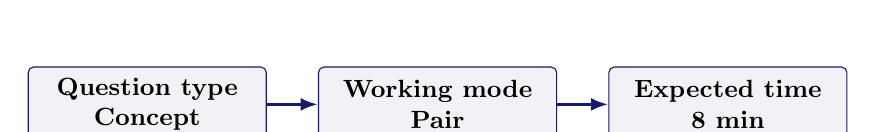
\begin{tikzpicture}[
node distance=0.65cm,
box/.style={draw=MidnightBlue, rounded corners=2pt, minimum height=0.95cm, align=center, font=\small\bfseries, fill=MidnightBlue!6, text width=0.23\linewidth},
arrow/.style={-{Latex[length=2.2mm]}, very thick, MidnightBlue}
]
\node[box] (type) {Question type\\Concept};
\node[box, right=of type] (mode) {Working mode\\Pair};
\node[box, right=of mode] (time) {Expected time\\8 min};
\draw[arrow] (type) -- (mode);
\draw[arrow] (mode) -- (time);
\end{tikzpicture}
\end{center}

{\large\bfseries\color{MidnightBlue} Prompt}\par\medskip
Start with the question from the lecture opener: How do babies learn to walk without step-by-step instructions? Use it to explain what trial and error, feedback, and improvement over time mean in reinforcement learning.

{\large\bfseries\color{MidnightBlue} Task details}\par\medskip
\begin{itemize}\item \textbf{Type:} concept
\item \textbf{Mode:} pair
\item \textbf{Time:} 8 min
\item \textbf{Deliverable:} short explanation
\item \textbf{Assessment focus:} connect everyday trial-and-error learning to the core RL idea
\item \textbf{Expected length:} 3 bullets + 1 example\end{itemize}

{\large\bfseries\color{MidnightBlue} How to submit}\par\medskip
Post one pair Padlet comment with three short bullets and one everyday example besides walking.

{\large\bfseries\color{MidnightBlue} Discussion in class}\par\medskip
Which part of this story is most similar to delayed reward?

{\large\bfseries\color{MidnightBlue} Why this helps}\par\medskip
Useful for short introductory questions that ask what reinforcement learning is trying to do.

{\large\bfseries\color{MidnightBlue} References}\par\medskip
\begin{itemize}\item Russell \& Norvig (2021) AIMA 4e, Ch.22, pp.789-822
\item Poole \& Mackworth (2023) 3e, Ch.13, pp.583-608\end{itemize}
\end{tcolorbox}

\begin{tcolorbox}[colback=white,colframe=MidnightBlue,title={Q2 Core Concept Check},fonttitle=\bfseries,breakable]
\begin{center}
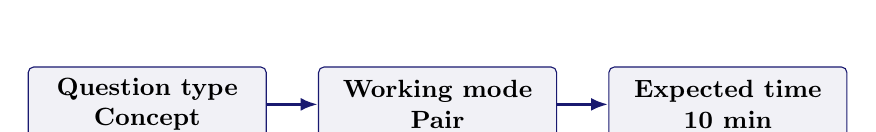
\begin{tikzpicture}[
node distance=0.65cm,
box/.style={draw=MidnightBlue, rounded corners=2pt, minimum height=0.95cm, align=center, font=\small\bfseries, fill=MidnightBlue!6, text width=0.23\linewidth},
arrow/.style={-{Latex[length=2.2mm]}, very thick, MidnightBlue}
]
\node[box] (type) {Question type\\Concept};
\node[box, right=of type] (mode) {Working mode\\Pair};
\node[box, right=of mode] (time) {Expected time\\10 min};
\draw[arrow] (type) -- (mode);
\draw[arrow] (mode) -- (time);
\end{tikzpicture}
\end{center}

{\large\bfseries\color{MidnightBlue} Prompt}\par\medskip
Compare reinforcement learning and supervised learning using the three lecture ideas of feedback timing, how training data is collected, and what objective is optimised. Finish with one real example where reinforcement learning is the better fit.

{\large\bfseries\color{MidnightBlue} Task details}\par\medskip
\begin{itemize}\item \textbf{Type:} concept
\item \textbf{Mode:} pair
\item \textbf{Time:} 10 min
\item \textbf{Deliverable:} comparison bullets
\item \textbf{Assessment focus:} distinguish reinforcement learning from supervised learning using day-1 concepts
\item \textbf{Expected length:} 4 bullets + 1 example\end{itemize}

{\large\bfseries\color{MidnightBlue} How to submit}\par\medskip
Post one pair Padlet comment with one bullet for each contrast and one example.

{\large\bfseries\color{MidnightBlue} Discussion in class}\par\medskip
Which contrast matters most when the agent must act in the real world?

{\large\bfseries\color{MidnightBlue} Why this helps}\par\medskip
Useful for theory questions that ask for a direct comparison between learning paradigms.

{\large\bfseries\color{MidnightBlue} References}\par\medskip
\begin{itemize}\item Russell \& Norvig (2021) AIMA 4e, Ch.22, pp.789-822
\item Poole \& Mackworth (2023) 3e, Ch.13, pp.583-608\end{itemize}
\end{tcolorbox}

\begin{tcolorbox}[colback=white,colframe=MidnightBlue,title={Q3 Structured Problem},fonttitle=\bfseries,breakable]
\begin{center}
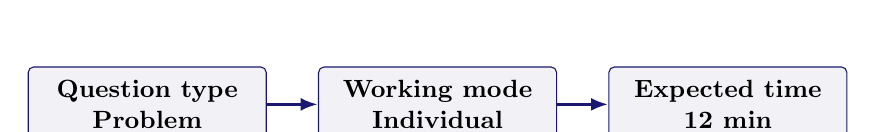
\begin{tikzpicture}[
node distance=0.65cm,
box/.style={draw=MidnightBlue, rounded corners=2pt, minimum height=0.95cm, align=center, font=\small\bfseries, fill=MidnightBlue!6, text width=0.23\linewidth},
arrow/.style={-{Latex[length=2.2mm]}, very thick, MidnightBlue}
]
\node[box] (type) {Question type\\Problem};
\node[box, right=of type] (mode) {Working mode\\Individual};
\node[box, right=of mode] (time) {Expected time\\12 min};
\draw[arrow] (type) -- (mode);
\draw[arrow] (mode) -- (time);
\end{tikzpicture}
\end{center}

{\large\bfseries\color{MidnightBlue} Prompt}\par\medskip
In a smart-greenhouse control task, the agent is in state g4, takes action Heat, receives reward -1, moves to state g5, and currently has Q(g4, Heat)=2.4, max\_a Q(g5,a)=6.0, alpha=0.5, gamma=0.8. Identify the state, action, reward, and next state, then compute the updated Q(g4, Heat).

\begin{tcolorbox}[colback=ForestGreen!5,colframe=ForestGreen,title={Formula reminder},fonttitle=\bfseries,breakable]
\[
Q_{\text{new}}(s,a)=Q(s,a)+\alpha\left[r+\gamma \max_{a'}Q(s',a')-Q(s,a)\right]
\]
\textbf{Use this when the task asks for one update step.}
\end{tcolorbox}

{\large\bfseries\color{MidnightBlue} Task details}\par\medskip
\begin{itemize}\item \textbf{Type:} problem
\item \textbf{Mode:} individual
\item \textbf{Time:} 12 min
\item \textbf{Deliverable:} worked update
\item \textbf{Assessment focus:} identify RL elements correctly and execute one Q-learning update
\item \textbf{Expected length:} 4 labels + 4 calculation lines\end{itemize}

{\large\bfseries\color{MidnightBlue} How to submit}\par\medskip
Post your own Padlet comment showing the four RL elements, the substitution into the update rule, the target, and the final value.

{\large\bfseries\color{MidnightBlue} Discussion in class}\par\medskip
Which quantity in the update says what the agent expects from the next state?

{\large\bfseries\color{MidnightBlue} Why this helps}\par\medskip
Direct practice for state-action-reward identification and Q-learning calculations.

{\large\bfseries\color{MidnightBlue} References}\par\medskip
\begin{itemize}\item Russell \& Norvig (2021) AIMA 4e, Ch.22, pp.789-822
\item Poole \& Mackworth (2023) 3e, Ch.13, pp.583-608\end{itemize}
\end{tcolorbox}

\begin{tcolorbox}[colback=white,colframe=MidnightBlue,title={Q4 Stretch Extension},fonttitle=\bfseries,breakable]
\begin{center}
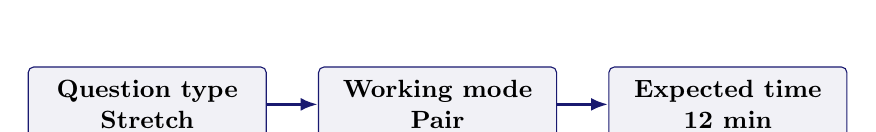
\begin{tikzpicture}[
node distance=0.65cm,
box/.style={draw=MidnightBlue, rounded corners=2pt, minimum height=0.95cm, align=center, font=\small\bfseries, fill=MidnightBlue!6, text width=0.23\linewidth},
arrow/.style={-{Latex[length=2.2mm]}, very thick, MidnightBlue}
]
\node[box] (type) {Question type\\Stretch};
\node[box, right=of type] (mode) {Working mode\\Pair};
\node[box, right=of mode] (time) {Expected time\\12 min};
\draw[arrow] (type) -- (mode);
\draw[arrow] (mode) -- (time);
\end{tikzpicture}
\end{center}

{\large\bfseries\color{MidnightBlue} Prompt}\par\medskip
Using the lecture ideas about reward signals, delayed reward, learning rate, and discounting, answer these four linked questions: What happens to Q-values if rewards are always 0? What happens if rewards only arrive after many steps? What does a larger alpha change? What does a larger gamma change?

{\large\bfseries\color{MidnightBlue} Task details}\par\medskip
\begin{itemize}\item \textbf{Type:} stretch
\item \textbf{Mode:} pair
\item \textbf{Time:} 12 min
\item \textbf{Deliverable:} short analytical note
\item \textbf{Assessment focus:} reason about zero reward, delayed reward, and the roles of alpha and gamma
\item \textbf{Expected length:} 4 numbered answers\end{itemize}

{\large\bfseries\color{MidnightBlue} How to submit}\par\medskip
Post one pair Padlet comment with four numbered answers in simple language.

{\large\bfseries\color{MidnightBlue} Discussion in class}\par\medskip
Which setting makes learning look slow even when the update rule is correct?

{\large\bfseries\color{MidnightBlue} Why this helps}\par\medskip
Good extension for explanation questions about delayed reward, discounting, and learning-rate effects.

{\large\bfseries\color{MidnightBlue} References}\par\medskip
\begin{itemize}\item Russell \& Norvig (2021) AIMA 4e, Ch.22, pp.789-822
\item Poole \& Mackworth (2023) 3e, Ch.13, pp.583-608\end{itemize}
\end{tcolorbox}

\begin{tcolorbox}[colback=white,colframe=MidnightBlue,title={Q5 Collaborative Mini-Case},fonttitle=\bfseries,breakable]
\begin{center}
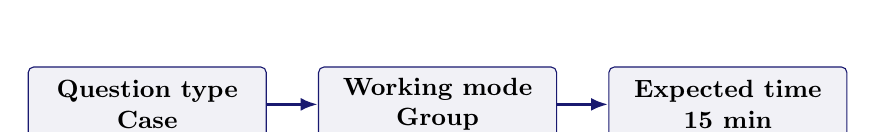
\begin{tikzpicture}[
node distance=0.65cm,
box/.style={draw=MidnightBlue, rounded corners=2pt, minimum height=0.95cm, align=center, font=\small\bfseries, fill=MidnightBlue!6, text width=0.23\linewidth},
arrow/.style={-{Latex[length=2.2mm]}, very thick, MidnightBlue}
]
\node[box] (type) {Question type\\Case};
\node[box, right=of type] (mode) {Working mode\\Group};
\node[box, right=of mode] (time) {Expected time\\15 min};
\draw[arrow] (type) -- (mode);
\draw[arrow] (mode) -- (time);
\end{tikzpicture}
\end{center}

{\large\bfseries\color{MidnightBlue} Prompt}\par\medskip
Imagine a tea-serving robot that learns by trial and error. Design a reward function that encourages task completion, avoids spills, avoids burns, and avoids wasting ingredients. Then add two controls that reduce reward hacking.

{\large\bfseries\color{MidnightBlue} Task details}\par\medskip
\begin{itemize}\item \textbf{Type:} case
\item \textbf{Mode:} group
\item \textbf{Time:} 15 min
\item \textbf{Deliverable:} reward-design sketch
\item \textbf{Assessment focus:} design a reward function with both task and safety terms
\item \textbf{Expected length:} 4 reward terms + 2 anti-hacking controls\end{itemize}

{\large\bfseries\color{MidnightBlue} How to submit}\par\medskip
Post one group Padlet comment with four reward terms, their signs or weights, and two anti-hacking controls.

{\large\bfseries\color{MidnightBlue} Discussion in class}\par\medskip
Which unsafe shortcut would your robot still try first if the reward is badly designed?

{\large\bfseries\color{MidnightBlue} Why this helps}\par\medskip
Supports design questions on reward specification, safety, and unintended behaviour.

{\large\bfseries\color{MidnightBlue} References}\par\medskip
\begin{itemize}\item Russell \& Norvig (2021) AIMA 4e, Ch.22, pp.789-822
\item Poole \& Mackworth (2023) 3e, Ch.13, pp.583-608\end{itemize}
\end{tcolorbox}

\begin{tcolorbox}[colback=white,colframe=MidnightBlue,title={Q6 Exam-Style Constructed Response},fonttitle=\bfseries,breakable]
\begin{center}
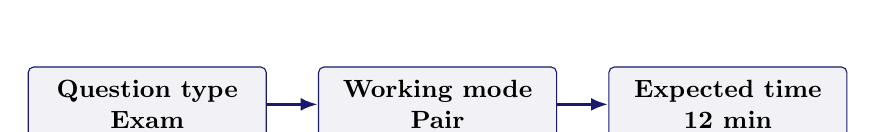
\begin{tikzpicture}[
node distance=0.65cm,
box/.style={draw=MidnightBlue, rounded corners=2pt, minimum height=0.95cm, align=center, font=\small\bfseries, fill=MidnightBlue!6, text width=0.23\linewidth},
arrow/.style={-{Latex[length=2.2mm]}, very thick, MidnightBlue}
]
\node[box] (type) {Question type\\Exam};
\node[box, right=of type] (mode) {Working mode\\Pair};
\node[box, right=of mode] (time) {Expected time\\12 min};
\draw[arrow] (type) -- (mode);
\draw[arrow] (mode) -- (time);
\end{tikzpicture}
\end{center}

{\large\bfseries\color{MidnightBlue} Prompt}\par\medskip
A hospital cleaning robot first learns in simulation and then fine-tunes in a real corridor where patients and staff may appear unexpectedly. Recommend a safer training setup for the real-world stage. Your answer must say whether learning should continue online or switch to evaluation-only deployment, and it must include one exploration control and one stop condition that would halt unsafe behaviour.

{\large\bfseries\color{MidnightBlue} Task details}\par\medskip
\begin{itemize}\item \textbf{Type:} exam
\item \textbf{Mode:} pair
\item \textbf{Time:} 12 min
\item \textbf{Deliverable:} claim-evidence-justification response
\item \textbf{Assessment focus:} justify a safer RL training setup under noise and human-safety constraints
\item \textbf{Expected length:} 180-240 words\end{itemize}

{\large\bfseries\color{MidnightBlue} How to submit}\par\medskip
Post one pair Padlet comment with a clear recommendation, two technical reasons, one exploration control, and one stop condition.

{\large\bfseries\color{MidnightBlue} Discussion in class}\par\medskip
Which safety control matters more in the real corridor: limiting exploration or stopping unsafe episodes quickly?

{\large\bfseries\color{MidnightBlue} Why this helps}\par\medskip
Matches longer answers that ask for training trade-offs, deployment safety, and practical RL guardrails.

{\large\bfseries\color{MidnightBlue} References}\par\medskip
\begin{itemize}\item Russell \& Norvig (2021) AIMA 4e, Ch.22, pp.789-822
\item Poole \& Mackworth (2023) 3e, Ch.13, pp.583-608\end{itemize}
\end{tcolorbox}

\section*{Submission Instructions}

Use the seeded Padlet posts for Q1--Q6. Q3 is individual. Q1, Q2, Q4, and Q6 are pair tasks. Q5 should be one joint group comment. Start each comment with your names or group label.

\section*{Whole-Class Debrief Prompts}

\begin{itemize}
\tightlist
\item
  Which part of everyday trial-and-error learning maps most directly to reinforcement learning?
\item
  What makes delayed reward harder than immediate reward?
\item
  Which reward-design mistake is most likely to cause unsafe behaviour?
\end{itemize}

\section*{Exam Transfer Note (Day-Level)}

Maps to exam questions on RL intuition, delayed reward, Q-learning updates, parameter effects, reward design, and safety-aware method choice.

\end{document}
